\documentclass{beamer}

\usepackage{emoji}
\usepackage{tikz}

\usetikzlibrary{arrows.meta}
\usetikzlibrary{calc}

\usetheme{PSY9511}

\title{Russell's Paradox}
\author{Esten H. Leonardsen}
\date{10.02.25}


\begin{document}
	\begin{frame}
	 	\maketitle
	\end{frame}

    \begin{frame}{Background}
        \begin{tikzpicture}
            \node[] at (-5.25, -3.5) {};
            \node[] at (5.25, 3.5) {};

            \visible<1-2>{
                \node[inner sep=0pt, draw=black, rotate=90] at (-2.675, 0) {
                    \includegraphics[width=5cm]{data/tattoo.jpg}
                };
            }
            \visible<2>{
                \node[] at (2.675, 0) {
                    $\{S | S \notin S\}$
                };
            }
            \visible<3>{
                \node[inner sep=0pt, draw=black, label=below:\tiny{Source: A guy I met at a party once}] at (0, 0) {
                    
\includegraphics[width=9cm]{data/westworld.jpg}
                };
            }
        \end{tikzpicture}
    \end{frame}

    \begin{frame}{Historical underpinnings}
        \begin{tikzpicture}
            \node[draw=black] at (-5.25, -3.5) {};
            \node[draw=black] at (5.25, 3.5) {};

            \visible<1>{
                \node[inner sep=0pt, draw=black] at (0, 0) {
                    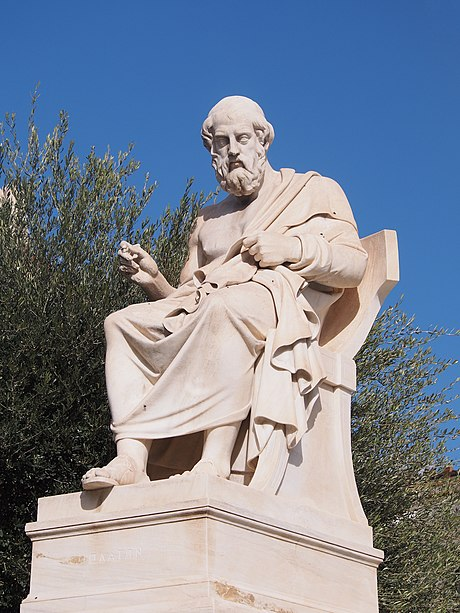
\includegraphics[width=4.5cm]{data/plato.JPG}
                };
            }
            \visible<2>{
                \node[inner sep=0pt, draw=black] at (0, 0) {
                    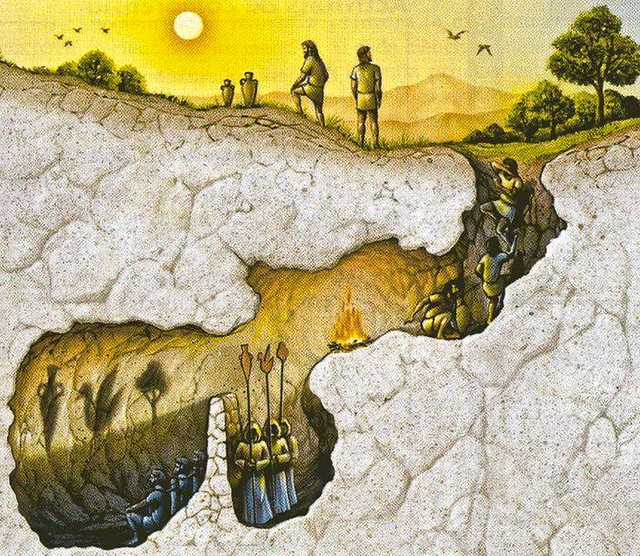
\includegraphics[width=7.5cm]{data/cave.jpg}
                };
            }
            \visible<3>{
                \node[inner sep=0pt, draw=black] at (0, 0) {
                    
\includegraphics[width=6cm]{data/kant.jpeg}
                };
            }
            \visible<4-5>{
                \node[inner sep=0pt, draw=black] at (-2.675, 0) {
                    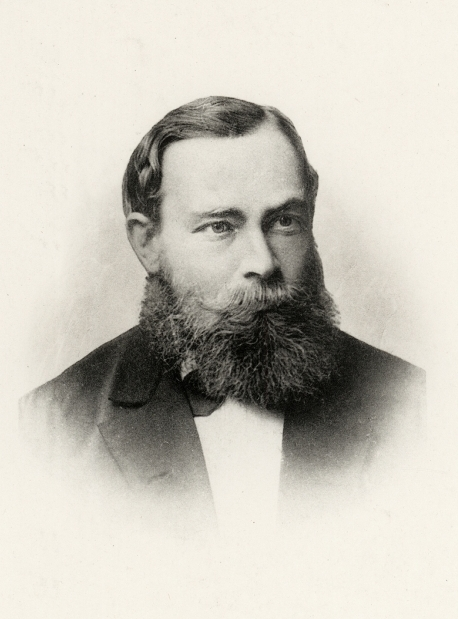
\includegraphics[height=5cm]{data/frege.jpg}
                };
            }
            \visible<5>{
                \node[inner sep=0pt, draw=black] at (2.675, 0) {
                    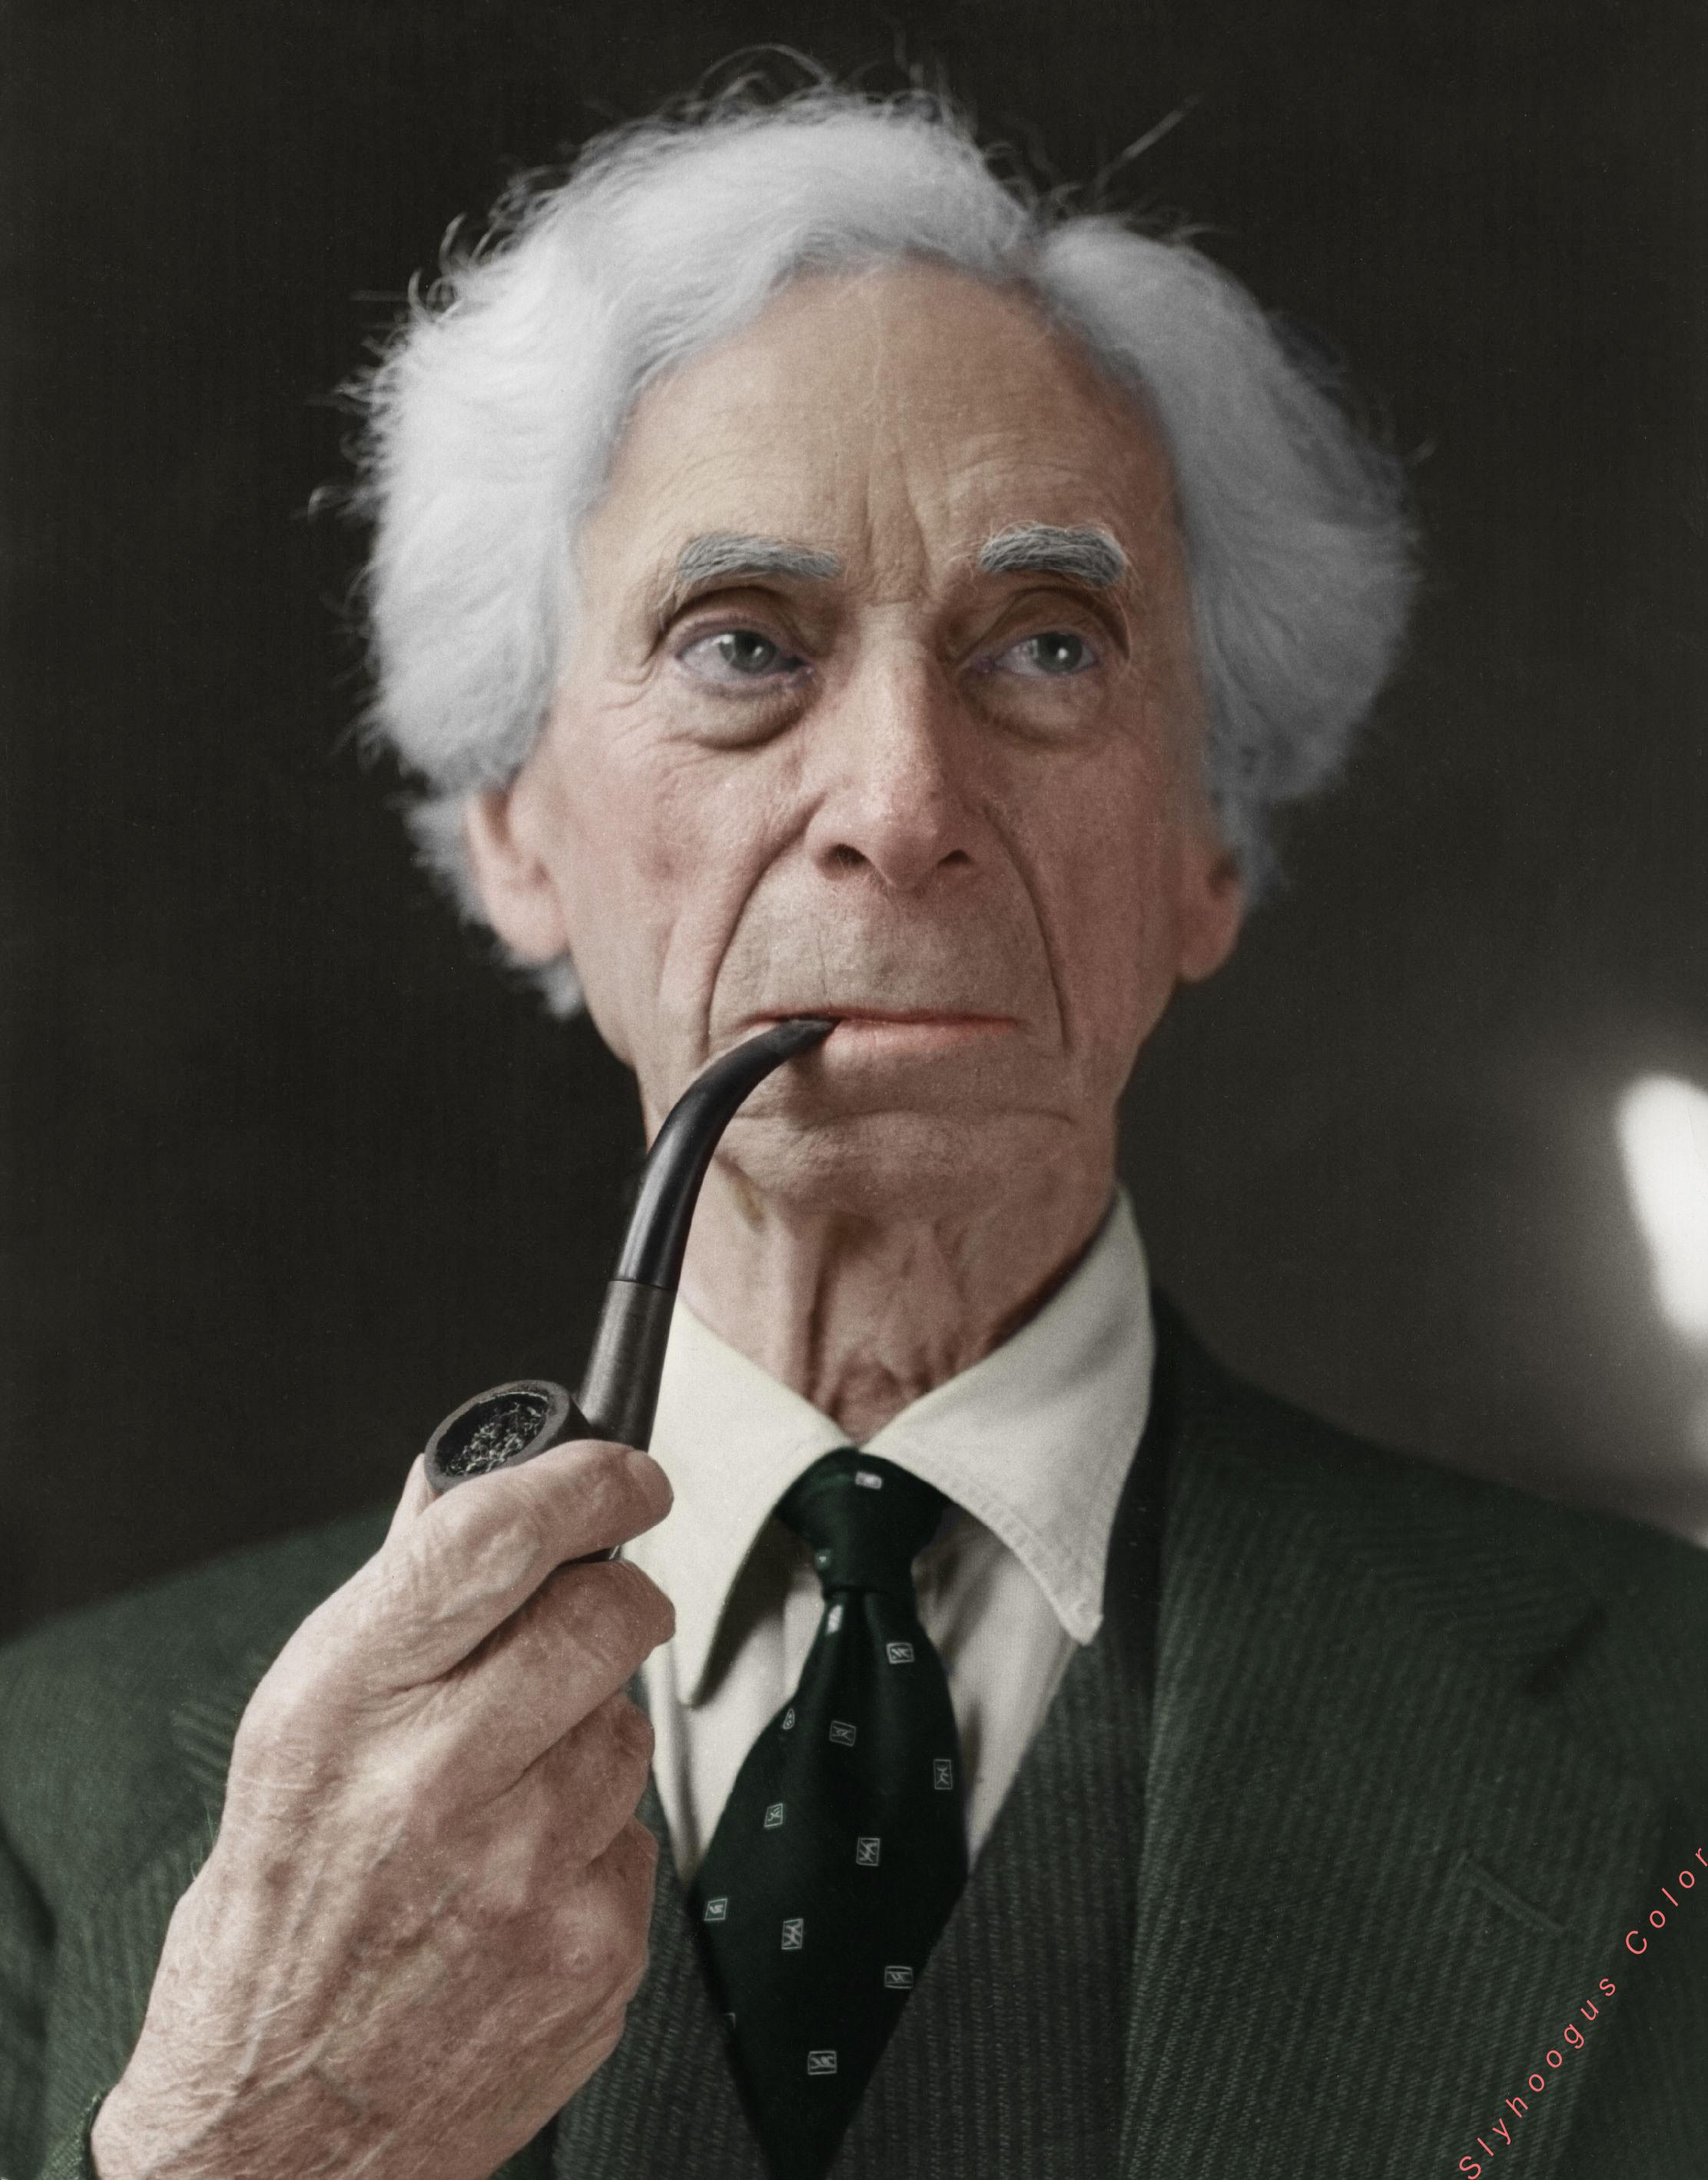
\includegraphics[height=5cm]{data/russell.jpg}
                };
            }
        \end{tikzpicture}
    \end{frame}

    \begin{frame}{The project}
        \begin{tikzpicture}
            \node[] at (-5.25, -3.5) {};
            \node[] at (5.25, 3.5) {};

            \visible<1-2>{
                \node[align=center] (functions) at (-2.675, -1) {
                    $x+y=z$\\$x-y=z$\\\ldots
                };
                \node[] (numbers) at (-2.675, 1) {
                    $0, 1, 2, 3, 4, \ldots$
                };
            }
            \visible<2>{
                \node[] at (0, 1) {
                    $\implies$
                };
                \node[] at (0, -1) {
                    $\implies$
                };
                \node[] at (2.675, 1) {
                    \large{\emoji{thinking-face}}
                };
                \node[] at (2.675, -1) {
                    \large{\emoji{check-mark-button}}
                };
            }
        \end{tikzpicture}
    \end{frame}

    \begin{frame}{Set theory}
        \begin{tikzpicture}
            \node[] at (-5.25, -3.5) {};
            \node[] at (5.25, 3.5) {};

            \visible<1>{
                \node[inner sep=0pt, draw=black] at (0, 0) {
                    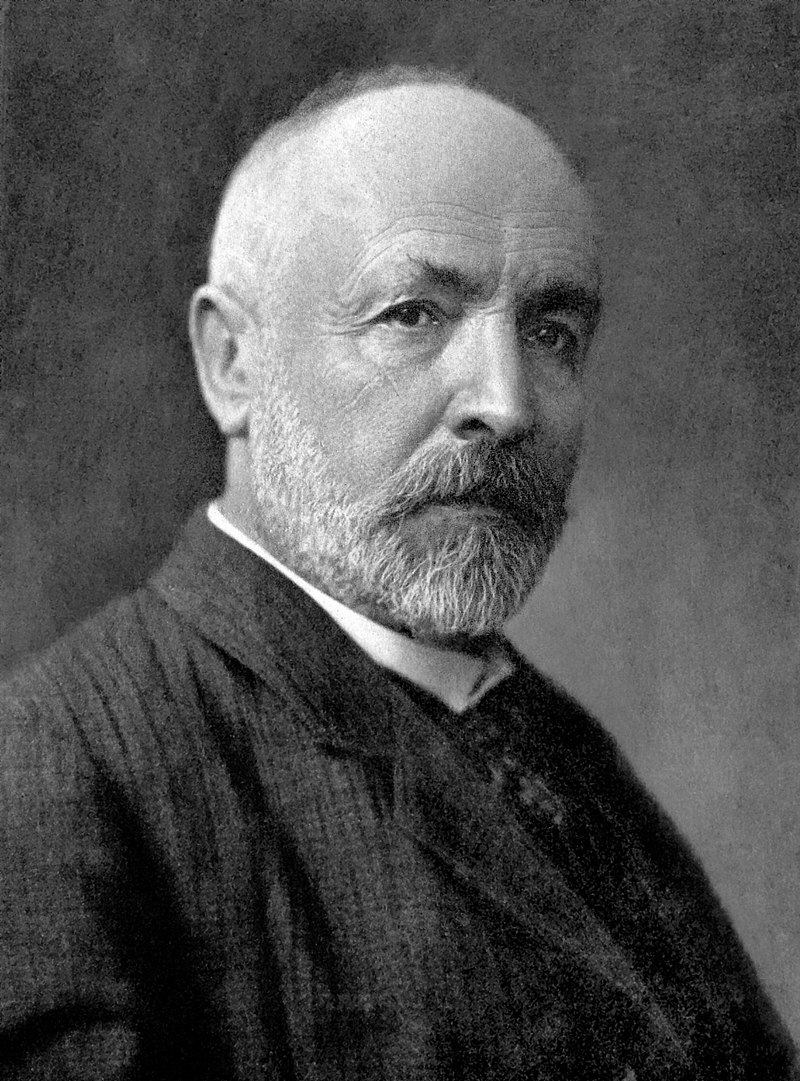
\includegraphics[width=5cm]{data/cantor.jpg}
                };
            }
            \visible<2>{
                \node[] at (0, 1.5) {
                    \{\emoji{nerd-face}, \emoji{woman}, \emoji{girl}, \emoji{dog-face}\}
                };
                \node[] at (0, 0.5) {
                    \{\emoji{nerd-face}, \emoji{smiling-face-with-sunglasses}, \emoji{face-with-monocle}, \emoji{woman-scientist},
                    \emoji{woman-technologist}, \emoji{woman-teacher}\}
                };
                \node[align=center] at (0, -0.5) {
                    \{monday, tuesday, wednesday, thursday,\\friday, saturday, sunday\}
                };
                \node[] at (0, -1.5) {
                    \{\emoji{laptop}, \emoji{mobile-phone}\}
                };
            }
            \visible<4>{
                \node[] at (0, 1) {
                    $\{1, 3, 5\}$
                };
                \node[] at (0, 0) {
                    $\{1, 10, 100\}$
                };
                \node[align=center] at (0, -1) {
                    $\{\}$
                };
            }
            \visible<5-6>{
                \node[] at (0, 0.5) {
                    $\{1, 2, 3, \ldots\}$
                };
            }
            \visible<6>{
                \node[] at (0, -0.5) {
                    $\{x\ |\ x > 0\}$
                };
            }
            \visible<7>{
                \node[] at (0, 0.5) {
                    $\{1, 3, 5, \ldots\}$
                };
                \node[] at (0, -0.5) {
                    $\{x\ |\ x\ \%\ 2\neq0\}$
                };
            }
            \visible<8-12>{
                \node[align=center] at (0, 1.5) {
                    \{\{\emoji{nerd-face}, \emoji{woman}, \emoji{girl}, \emoji{dog-face}\}, \{\emoji{nerd-face}, \emoji{smiling-face-with-sunglasses}, \emoji{face-with-monocle}, \emoji{woman-scientist},
                    \emoji{woman-technologist}, \emoji{woman-teacher}\},\\\{monday, tuesday, wednesday, thursday, friday, saturday, sunday\},\\\{\emoji{laptop}, \emoji{mobile-phone}\}, $\{1, 3, 5\}$, $\{1, 10, 100\}$, $\{\}$, $\{x\ |\ x > 0\}$, $\{x\ |\ x\ \%\ 2\neq0\}$\}
                };
            }
            \visible<9-12>{
                \node[] at (0, 0) {
                    $\{\{\}, \{0\}, \{1\}, \{0, 1\}, \ldots\}$
                };
            }
            \visible<10-12>{
                \node[] (s) at (0, -1) {
                    $\{x\ |\ x \mathrm{\ is\ a\ set}\}$
                };
            }
            \visible<11-12>{
                \node[anchor=east] at ($ (s.west) + (0.2, 0) $) {
                    $S=$
                };
            }
            \visible<12>{
                \node[] at (0, -2) {
                    $S \in S\ ?$
                };
            }
            \visible<13-16>{
                \node[] at (-2.5, 1) {
                    $S=\{\{\}, \{0\}, \{1\}, \{0, 1\}, \ldots, S, \ldots\}$
                };
                \node[] at (-2.5, 0) {
                    $S \in S$
                };
            }
            \visible<14-16>{
                \node[] at (2.5, 1) {
                    $S=\{1, 3, 5\}$
                };
                \node[] at (2.5, 0) {
                    $S \notin S$
                };
            }
            \visible<15-16>{
                \node[] at (0, -1.5) {
                    $\{S\ |\ S \in S\}$
                };
            }
            \visible<16>{
                \node[] at (0, -2) {
                    $\{S\ |\ S \notin S\}$
                };
            }

            \visible<17-22>{
                \node[] at (0, 1.5) {
                    $T=\{S\ |\ S \notin S\}$
                };
            }
            \visible<18-22>{
                \node[] (q) at (0, 0.5) {
                    $T \in T\ ?$
                };
            }
            \visible<19-22>{
                \node[] (no) at (-1.5, -1) {
                    No ($T \notin T$)
                };
                \draw[-stealth] (q) -- (no);
            }
            \visible<20-22>{
                \node[] (no2) at (-1.5, -2) {
                    Yes
                };
                \draw[-stealth] (no) -- (no2);
            }
            \visible<21-22>{
                \node[] (yes) at (1.5, -1) {
                    Yes ($T \in T$)
                };
                \draw[-stealth] (q) -- (yes);
            }
            \visible<22>{

                \node[] (yes2) at (1.5, -2) {
                    No
                };
                \draw[-stealth] (yes) -- (yes2);
            }
            \visible<23>{
                \node[inner sep=0pt, draw=black] at (0, 0) {
                    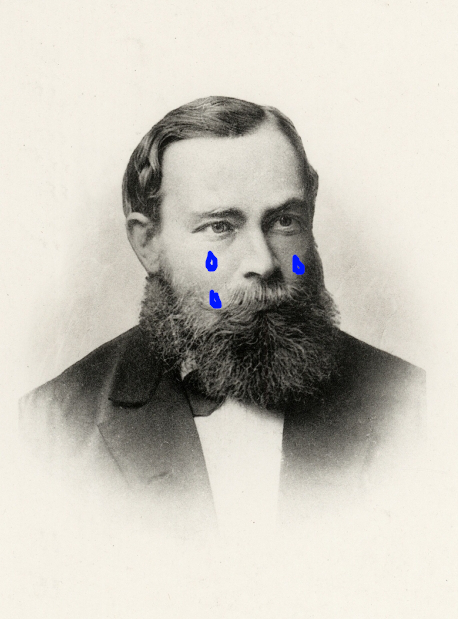
\includegraphics[height=6cm]{data/fregecry.jpg}
                };
            }
            \visible<24>{
                \node[align=center, text width=10cm, align=flush center] at (0, 0) {
                    \textit{"Hardly anything more unfortunate can befall a scientific writer than to have one of the foundations of his edifice shaken after the work is finished. This was the position I was placed in by a letter of Mr. Bertrand Russell, just when the printing of this volume was nearing its completion."}
                };
            }
        \end{tikzpicture}
    \end{frame}

    \begin{frame}{Later examples}
        \begin{tikzpicture}
            \node[] at (-5.25, -3.5) {};
            \node[] at (5.25, 3.5) {};

            \visible<1>{
                \node[inner sep=0pt, draw=black] at (0, 0) {
                    \includegraphics[width=6cm]{data/gødel.jpg}
                };
            }
        \end{tikzpicture}
    \end{frame}

\end{document}
